\documentclass{article}
\usepackage{CJKutf8}
\usepackage{multicol}
% Packages
\usepackage{lipsum} % For generating dummy text
\usepackage[top=1in, bottom=1in, left=1in, right=1in]{geometry}
\usepackage{hyperref}
\usepackage{pgfplots}
\usetikzlibrary{pgfplots.polar}
\usepackage{caption}
\captionsetup{font=small}
\usepackage{standalone}
\usepackage{listings}
\usepackage{xcolor} % For setting colors
\usepackage{amssymb}
\usepackage{amsmath}
\usepackage{algorithm}
\usepackage{algpseudocode}
\usepackage{afterpage}
\usepackage{placeins}
\usepackage{tikz}
\usepackage{enumitem}
\lstset{
  language=[LaTeX]TeX,
  breaklines=true,
  basicstyle=\ttfamily\small,
  keywordstyle=\color{blue},
  commentstyle=\color{green},
  backgroundcolor=\color{gray!10},
  frame=single,
  showspaces=false,
  showstringspaces=false,
}
\pgfplotsset{compat=1.17} % Use this to ensure compatibility with newer features
\setlength{\parskip}{6pt}
% Title and author

\title{Autonomous Competence Identification Protocol: A Dynamic Ranking Ladder System for Blockchain Applications}

\author{Tim Pechersky, Aivars Smirnovs}

\begin{document}
\begin{CJK}{UTF8}{gbsn}

    % \twocolumn
    \maketitle

    \begin{abstract}
        {{ This paper introduces the Autonomous Competence Identification Protocol (ACIP), a novel dynamic ranking ladder system designed for trustless environments. ACIP leverages game-theoretic principles and dynamic systems theory to autonomously identify and reward competence while effectively mitigating Sybil attacks. Participants compete in time-locked, tiered groups, progressing through ranks based on demonstrated competence. This protocol establishes a quantifiable, verifiable, and tokenized measure of competence, secured by time and financial commitment. ACIP offers a robust foundation for merit-based blockchain consensus, decentralized governance, and equitable online communities, moving beyond purely power-based systems. }}
    \end{abstract}

    \section{Introduction}

    Traditional meritocratic models struggle to objectively identify and reward competence.\cite{Arrow2000} This challenge is significantly amplified in decentralized systems, where trust is minimized and the risk of manipulation is high.  {{ Current decentralized systems often rely on Proof-of-Work or Proof-of-Stake, which primarily measure computational or financial resources rather than actual competence in governance or decision-making. This limitation hinders the development of robust and equitable decentralized governance and funding mechanisms, leading to concerns about the long-term viability of decentralized organizations. }} \cite{Rainer2023}\cite{Robin22}\cite{Xuan2024}

    This paper introduces a novel protocol to establish a dynamic ranking ladder system. Our protocol incentivizes participants to demonstrate their abilities through competitive "elections" within tiered groups. By requiring time and financial commitment, we create a system resistant to Sybil attacks and foster genuine competence development. This approach can be applied to various decentralized systems, including blockchain consensus mechanisms, contributing to more robust and equitable governance.

    Empirically, the protocol's dynamics can be observed in many online games. In these games, participants engage in competitions, and winners emerge through a process that inherently validates the protocol's core principles.

    This research aims to:

    \begin{itemize}[nosep]
        \item Propose a methodology for creating a dynamic ranking system in a trustless environment.
        \item Analyze attack vectors and present robust resistance mechanisms.
        \item Discuss applications and benefits of the competence framework.
    \end{itemize}

    The proposed protocol is a theoretical construct that relies on established consensus mechanisms to operate. It can be executed on existing blockchain protocols.

    \section{Protocol Mechanism}

    The Autonomous Competence Identification Protocol (ACIP) establishes a dynamic ranking ladder through a series of tiered groups and competitive interactions. Participants progress through ranks by demonstrating competence within these groups. The core components of the protocol are time-based participation and cost-based commitment, ensuring robustness and Sybil resistance.

        {{ The protocol operates through the following steps: }}

    \begin{enumerate}
        \item \textbf{Group Formation:} Participants join groups based on shared interests or topics. Groups are tiered, representing different levels of competence.
        \item \textbf{Time-Locked Participation:}  Participation in a group requires a time commitment ($T_{id}$), ensuring sustained engagement.
        \item \textbf{Cost-Based Commitment:} Joining a group and progressing in rank requires a financial stake ($X_{id}$), deterring Sybil attacks and frivolous participation.
        \item \textbf{Competitive Interaction ("Elections"):} Within each group, participants engage in a competitive process (e.g., voting, proposal evaluation, debate) to identify the most competent individuals. The specifics of this process are application-dependent.
        \item \textbf{Rank Advancement:} Winners of the competitive process within a group advance to higher ranks, reflecting their demonstrated competence. Losers remain in their current rank or may descend based on protocol rules.
        \item \textbf{Dynamic Rank Adjustment:} Ranks are not static; they are dynamically adjusted based on ongoing participation and performance in group competitions.
        \item \textbf{Competence Representation:}  Rank $R$ is represented and stored on-chain, providing a verifiable and transparent measure of competence. This rank can be tokenized or used as a reputation score within the decentralized system.
    \end{enumerate}

    This dynamic process creates a self-regulating ranking ladder where competence is continuously assessed and rewarded. The time and cost components ensure that rank is not easily gained through manipulation or superficial effort.

    \section{Protocol description}

    The protocol breaks participants into smaller groups to elect a winner. This election can be implemented as any sub-protocol like a block building challenge, community discussion, or general data exchange, which isn't discussed here. It involves multiple participants agreeing on a verifiable leader.

    We introduce two principal constant values for our protocol to make groups interoperable based on the same trust assumptions, yet free to define their own participation parameters: (1) principal time constant $P_t$ and (2) principal asset cost $P_c$. These create a common price and time relationship between groups. We also add a boundary case limitation $N_{min}$ - minimum number of participants required to form a group.

    Besides protocol-wide constants, we allow each group to have its own properties:
    \pagebreak
    \begin{itemize}[nosep]
        \item id - a protocol-wide unique group identifier
        \item $N$ - number of participants
        \item $T$ - minimum time agreed by members to finalize election
        \item $R$ - rank
        \item $S$ - state - can be:
              \begin{itemize}[nosep]
                  \item \textbf{created} - group is created and waiting for participants.
                  \item \textbf{started} - group starts $ts_i$ time of start is recorded
                  \item \textbf{finalized} - group is finalized
              \end{itemize}
              % \item $X$ - stake requirement
    \end{itemize}

    Additionally, there are two global properties for each participant:

    \begin{itemize}[nosep]
        \item  $P_r$ - participant
        \item $P_g$ - group id last joined by participant
    \end{itemize}

    Participants can change groups only if their current and target group are not in "started" state. Whenever someone starts a group, it must have at least $N_{min}$ participants and result in an irreversible stake of participation $X_{id}$ to all participants' balance:
    \begin{equation}
        \label{eq:group-fee}
        X_{id} = f(T_{id}) = \dfrac{P_t \cdot  P_c }{T_{id}}
    \end{equation}

    These costs can be broken down into equal stakes subtracted from each participant's account whenever group changes its state to "started":
    \begin{equation}
        \label{eq:join-fee}
        stake = \dfrac{X_{id}}{ N_{id}}
    \end{equation}
    \input{ladder.tex}
    The concept of "irreversible" implies that no participant of group is getting back their stake at full value. This is a key feature of the protocol that ensures the ranking system isn't manipulated by financial power. The stake instead can be channeled for protocol utility operations, data retention in case of storage heavy applications like \cite{cvpp} may be. The partial stake may be used as a reward pool for the winners, however in such case collusion resistance is lowered and additional collision mechanisms, such as proof of humanity \cite{WorldCoin2024} combined with advising participants on collusion attack risks within a groups they join, or similar, are desired.



    The group can finalize only after $T_{i}$ has elapsed since the start state transition and start transition must be recorded on the underlying consensus or similar, guaranteeing the visibility of the start transition for other ranking ladder competitors globally.

    A winner can be declared and his rank $P_r$ in the state trie incremented to $P_r=P_r+1$ only if group rank $R$ equals $P_r$ before finalization. This process can repeat and is illustrated in Fig. \ref*{fig:game-connection}.

    \paragraph{Dynamic Proof-of-Authority.} The state transfer is unidirectional from assets to rank and time-dependent. This makes every transition to incur cost equal to a differential equation:

    \begin{equation}
        \label{eq:time-weighted-proof-of-authority}
        \$P_r = \$(P_r-1) + X_{id}
    \end{equation}
    While the maximal rate of obtaining any rank $P_r$ is a unit step function dependent on time $t$:
    \begin{equation}
        \label{eq:time-weighted-proof-of-authority-1}
        T_{\Delta Pr}(t,id) = \lfloor \dfrac{t \cdot P_t \cdot P_c}{T(id)} \rfloor
    \end{equation}

    Where $T_{\Delta Pr}$ is a time required to obtain a rank difference of 1. Substituting  the \ref{eq:group-fee} equation into \ref{eq:time-weighted-proof-of-authority-1} gives clear "time money" relationship.

    \begin{equation}
        \label{eq:time-weighted-proof-of-authority-2}
        T_{\Delta Pr}(t,id) = \lfloor X_{id} \cdot t \rfloor
    \end{equation}

    \paragraph*{Frequency domain.} Eq. \ref{eq:time-weighted-proof-of-authority-1} highlights the dynamic nature of the protocol. Since it shows linear-time invariant property, the dynamic systems theory \cite{Lynn86} may be applied to analyze its stability and predict its future behavior. ${T(id)}$ is a specific minimal time to finalize a group election of group ${id}$.

    $1/T(id)$ represents frequency, hence phase and frequency relationships between groups exist. Analysis my be done in s-domain using Laplace transforms.

    Different groups (${id}$) with different ${T_{id}}$ would result in a dynamic competence ladder that can produce specific quorums at specific times and due to limited resources to stake and irreversible nature of the stake, even if quorum is achieved, it is temporary and accommodates for time division multiplexing between competing groups.

    \subsection{Dynamic Systems Theory and Protocol Behavior}

    The protocol's dynamic nature lends itself to analysis through dynamic systems theory.  {{ This theoretical framework helps to understand the time-evolving behavior of the ranking system, including stability, convergence, and response to external influences (e.g., influx of new participants, changes in participation costs).  Dynamic systems theory provides tools to model and predict how groups and individual ranks will evolve over time, especially in response to competitive interactions and potential adversarial behaviors. }}

    We can model the evolution of ranks and group dynamics using differential equations or agent-based simulation, considering factors such as participation rates, competition intensity, and Sybil attack attempts. This analysis can inform parameter tuning and protocol optimization to ensure desired system properties, such as rapid convergence to a stable ranking and resilience against manipulation.

    The time-based nature of the protocol introduces cyclical and oscillatory behaviors, particularly in how groups form and dissolve, and how participant engagement fluctuates over time.

    \section{Sybil Attack Resistance}

    The protocol's outcome represents an agent's competence by storing his $R$ rank in the state trie. To ensure this representation isn't manipulatable, we must analyze security concerns.

    From a game theory perspective, an adversary can be a group producing a winner with $R$ rank higher than any other group. However, the payment requirement in Eq. \ref{eq:group-fee} will be proportional to the number of participants, contrary to the stake requirement fair participants are expected to pay (Eq. \ref{eq:join-fee}).

    Principal components defining fees ensure any winner from any group is time and asset effort normalized.

    If $T_{id} = P_t$, then equation \ref{eq:group-fee} reduces to:

    \begin{equation}
        \label{eq:join-fee-2}
        X_{id} = P_c
    \end{equation}

    If one participant's rank $R$ transition requires a commitment from $N_{min}$ participants, such as a participation fee $X_{id}$, we can demonstrate that the proposed ranking ladder introduces a non-linear compounding friction for malicious actors attempting to manipulate the system. The strategy depends on the application of how the agents decide on the winner for such an adversary. If the process is deterministic, the expected cost is

    \begin{equation}\
        \label{eq:direct-sybil-cost}
        X_{id} \cdot N_{min}^R
    \end{equation}
    If an adversary can mix with fair non-sybil agents and the process is not fully deterministic, we can use the mathematical expectation for costs achieving specific rank via sybil attack described as
    \begin{equation}
        \label{eq:math-expectation-sybil-cost}
        \mathbb{E}[\$R] = X_{id} \cdot \mathbb{E}[N_{\text{sybils}}(R)]
    \end{equation}

    Where $N_{sybils}(R)$ is the number of sybil accounts required to take quorum in a group and obtain rank $R$.
    \paragraph{Actor likeliness and group fragmentation.}
    From Eq. \ref{eq:direct-sybil-cost}, higher groups are more expensive to manipulate. However, breaking them into smaller ones may be desired to prevent communication complexity.Due to such group fragmentation, an attacker willing to maximize his attack efficiency must allocate accounts across groups strategically.

    This observation implies that for a fully autonomous protocol implementation, where no extra proofs of humanity or anti-collusion mechanisms used, there is a need for what we coin as \textit{agent collusion clustering system}.

    This system, not necessarily part of protocol must ensure analytics and alerting, giving participants ability to assess the likelihood of a specific group being a sybil attack. If a group seems likely to be a sybil attack, participants must be able to opt out. This can be done by reviewing the past state history of participants, groups they are joining, and the social graph from vote allocation, using the dynamic systems methodology proposed in the previous section.

    The collusion clustering system acts as a visibility tool, providing warnings and insights to agents, empowering them to make informed decisions about group selection. The core of collusion resistance lies in the agent's ability to choose groups that are not corrupted against them.

        {{  Practically, this system could function as a dashboard or set of alerts that provide participants with information such as: }}
    \begin{itemize}
        \item \textbf{Group Composition History:} Visualizations of how group membership has changed over time, highlighting sudden influxes of new accounts.
        \item \textbf{Social Graph Analysis:}  Network graphs showing voting patterns and connections between accounts within a group and across groups, identifying unusually dense clusters that might indicate collusion.
        \item \textbf{Anomaly Detection Alerts:}  Automated alerts triggered by unusual patterns in participation, voting, or rank progression that deviate from expected behavior based on historical data and dynamic system models.
    \end{itemize}
    {{ Participants could use this information to assess the risk of joining a potentially Sybil-attacked group and make more informed decisions about where to allocate their time and stake. }}

    \subsection{Quorum Resonances}
    \label{sec:time-constraint}

    As discussed earlier, any overt Sybil attack requires multiple groups to establish a sufficient ranking within the system. The intrinsic value of a tokenized competence rating is determined by financial effort, peer success, and time invested in improving one's position. An attacker needs $t_{attack}(R) = t_c \cdot R$ time to reach rank $R$. This duration allows protocol members to detect and respond to the attack.

    The Eq. \ref{eq:time-weighted-proof-of-authority-1} shows that system can be analyzed in time and frequency domains. This allows Sybil attacks analysis based on time, phase, and complex frequency domain analysis.

    Given the initial goal to facilitate protocol for subjective reasoning, it's unclear what a "Sybil attack" or a "different opinion" is. Assuming different opinions exist, and using the proposed s-domain methodology, competing groups can create a quorum resonance, where the opinion direction can oscillate. It takes the same $T$ for competing groups starting their election process at phase difference of $\pi$. This can be visualized in plot \Ref{fig:processes}.:

    \begin{figure}[ht]
        \centering
        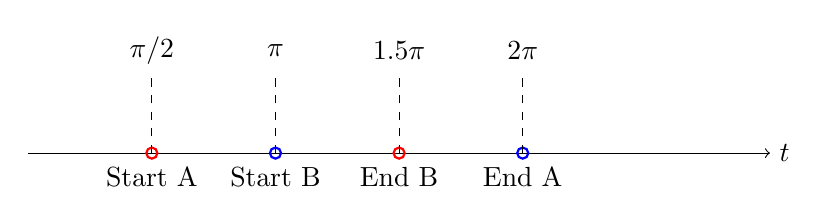
\begin{tikzpicture}
            % Define the x-axis
            \draw[->] (0,0) -- (3*3.14,0) node[right] {$t$};

            % Define the first process (point at Pi)
            \draw[blue, thick] (3.14,0) circle (2pt);
            \draw[blue, thick] (3.14*2,0) circle (2pt);
            \node[] at (3.14*0.5,1.3) {$\pi/2$};
            \node[] at (3.14,1.3) {$\pi$};
            \node[] at (3.14*1.5,1.3) {$1.5\pi$};
            \node[] at (3.14*2,1.3) {$2\pi$};

            % Define the second process (point at Pi/2)
            \draw[red, thick] (1.57,0) circle (2pt);
            \draw[red, thick] (1.57+3.14,0) circle (2pt);

            % Add labels for the timing diagram
            \node at (1.57,-0.3) {Start A};
            \node at (3.14,-0.3) {Start B};
            \node at (3.14*2,-0.3) {End A};
            \node at (1.57+3.14,-0.3) {End B};

            % Add dashed lines to indicate the timing
            \draw[dashed] (1.57,0) -- (1.57,1);
            \draw[dashed] (3.14,0) -- (3.14,1);
            \draw[dashed] (3.14*2,0) -- (3.14*2,1);
            \draw[dashed] (1.57+3.14,0) -- (1.57+3.14,1);
        \end{tikzpicture}
        \caption{Timing diagram showing two opposite opinion groups completing their election process at different times. The groups have the same $T$ with a phase difference of $\pi$, allowing opposite opinions to co-exist.}
        \label{fig:processes}
    \end{figure}

    If many groups allocate their reasoning power in alliance, more complicated systems can be imagined. These can create local quorum resonances, analyzable in frequency domain, to predict future behavior like illustrated in Fig. \ref{fig:processes-sinusoidal}.

    \begin{figure}[ht]
        \centering
        \begin{tikzpicture}
            % Define the x-axis
            \draw[->] (0,0) -- (10,0) node[right] {$T_{id1}=T_{id2}$};

            % Define the y-axis
            \draw[->] (0,-2) -- (0,2) node[above] {Quorum power};

            % Define the first process (sine wave)
            \draw[domain=0:10,smooth,variable=\t,blue] plot ({\t},{sin(360*\t/10)});
            \node[blue] at (10,1) {Quorum 1};

            % Define the second process (sine wave shifted by half period)
            \draw[domain=0:10,smooth,variable=\t,red] plot ({\t},{sin(360*\t/10 + 180)});
            \node[red] at (10,-1) {Quorum 2};

            % Add labels for the half period shift
            \draw[dashed] (5,-2) -- (5,2);
            \node at (5,-2.5) {$\pi$};

            % Add labels for the full period
            \draw[dashed] (10,-2) -- (10,2);
            \node at (10,-2.5) {$2\pi$};

        \end{tikzpicture}
        \caption{Diagram showing two competing opinion groups over the same subject with the same $T$ but a $\pi$ phase difference. Sinusoidal waves illustrate their ability to strategically allocate their ranking on the time axis. In reality, the groups may have different $T$ and could be more complex.
            \label{fig:processes-sinusoidal}}
    \end{figure}

    \subsection*{Utility of the allocated funds}
    The allocated funds can't be fully used to reward winners and must be locked in representation of rank $R$. If used in amount above mathematical expectation of sybil attack (Eq. \ref{eq:math-expectation-sybil-cost}) to reward winners, the system would be subject to manipulation by the highest bidder. This is a key feature of the protocol that ensures the ranking system isn't manipulated by financial power.

    The financial asset can fund any underlying protocol utility for the discussion. If used with CVPP\cite{cvpp}, the funds can guarantee data availability of the discussion in a specific group, ensuring transparency in Sybil attack resistance. Protocols allowing on-chain payments for long-term data availability like Swarm \cite{swarm} ensure data availability by allowing operators to pull budget from the group's account.

    The economic incentive for participation is rooted in the intrinsic interest of participants to engage in discussions about topics they are passionate about. Furthermore, the Total Value Locked (TVL) within the protocol enhances the value of the competence score, transforming it into a valuable reputation asset.

    We define competence within this protocol as: the measure of time and financial resources an individual is willing to commit, validated by the peer-assessed competence they receive in return for this investment.

        {{ Beyond data availability, locked funds could also be utilized for: }}
    \begin{itemize}
        \item \textbf{Funding Public Goods:}  Allocating a portion of funds to support development or maintenance of the protocol itself or related public goods.
        \item \textbf{Incentivizing Protocol Usage:}  Using funds to subsidize participation costs in certain groups or for specific types of contributions.
        \item \textbf{Community Governance:}  Potentially allowing holders of rank (and thus locked funds) to participate in governance decisions related to the protocol's operation and evolution.
    \end{itemize}
    {{ These potential utilities broaden the scope of the protocol and enhance its value proposition. }}

    \section{Conclusion}

    This paper introduces a novel protocol for establishing a dynamic ranking ladder system in trustless environments. Our protocol enables autonomous identification while mitigating Sybil attacks by leveraging game-theoretic principles and dynamic systems theory. The time-based and cost-based mechanisms ensure high ranks require genuine effort and skill, and opposite opinions can co-exist.

    This protocol offers a foundation for building more robust and equitable decentralized governance systems. It improves blockchain consensus mechanisms, enhances DAO decision-making, and fosters healthier online communities.

    Further work is needed to analyze the protocol's behavior and effectiveness using dynamic system theory and explore its integration with existing decentralized platforms.

    A need for agent collusion clustering system is proposed as auxiliary system to ensure increasing sybil attack resistance.

    Due to the principal components of time and cost, the protocol can support a large number of groups, ensuring maximized scalability and adaptability to diverse needs.

    A roadmap for integrating this protocol into existing decentralized platforms will be provided in follow-up works.

    The utility of locked funds is multifaceted: it is used to retain data about competitions, optionally serves as a funding source for protocol operations, and most importantly, functions as TVL locked within the representation of competence. This TVL allows the Proof of Competence to be quantified in both financial and temporal terms.

    In comparison to existing solutions, our protocol distinguishes itself by not enforcing specific KYC requirements and by using the social graph as an auxiliary tool for collusion clustering rather than a central component. This makes it a valuable and complementary addition to systems that rely on stricter identity verification methods.

        {{  Furthermore, unlike purely reputation-based systems that can be slow to adapt and vulnerable to initial bias, ACIP's dynamic ranking ladder offers a more responsive and continuously updated measure of competence.  Compared to systems relying solely on subjective peer review, ACIP introduces objective cost and time commitments, making competence harder to fake and easier to verify.  ACIP can be seen as complementary to existing decentralized identity and reputation solutions, providing a robust and dynamic competence layer that can enhance their effectiveness. }}

    \clearpage

    \bibliographystyle{ieeetr}
    \bibliography{../references.bib}

    \clearpage\end{CJK}
\end{document}
